\section{Visual-based Programming Languages}
\label{sec:visual_based_programming_languages}

Traditionally, most programming languages are categorized as text-based because of the way the program logic is written, by making use of a syntax, specific to every language. Therefore, it is often difficult to learn and use a programming language since it requires one to familiarize oneself with the syntax and available constructs first in order to use the language effectively and that takes skill many people lack. 

In order to address the difficulties in learning programming, for the past 50 years \cite{VisualProgHistory}, research has been done on the so called “Visual Programming” or “Graphical Programming”, and dozens of visual-based programming languages have been created. This approach, reserved and used in the past primarily for systems design, allows the use of spatial representations in two or more dimensions in the form of blocks and different structures and shapes. Compared to text-based programming where lines of code are used, graphical programming replaces these with visual objects, essentially replacing the textual representation of language components with a graphical one, more suitable for visual learners and intuitive for people with no prior knowledge in programming. The creation of programs in such languages is defined by placement and connection between visual objects where the syntax is encoded within the objects' shapes.  
The main aim of visual programming languages (VPL) and environments, as stated by Koitz ans Slany \cite{KoitzSlany14}, is “\textit{diminishing the syntactical burden and enabling a focus on the semantic aspects of coding}.” VPL try to facilitate end-user programming, both kids and adult novice programming, empowering the creation of new programs, not just their consumption, effectively minimising the distance between the cognitive and computational model.

Currently, there is a wide variety of visual programming languages with varying popularity such as Alice, Greenfoot, Tynker, Scratch, Raptor and many more. From these, Scratch and Alice will be described and analyzed further.

\subsection{Scratch}
Scratch is a visual-based programming environment which allows users to create visually-rich, interactive projects.  Since its inception in 2003, the main goal of its creators has been to address the needs and interests of young people (primarily ages 8 to 16) and make a soft introduction to the world of programming for them. Publicly released in 2007, the project has grown in size and scope, with a dedicated site hosting all its 11 million projects and with a user base of 8 million \cite{scratchstat}.
Given its targeted audience, one of the main design goals of Scratch is the focus on self-directed learning and exploration through tinkering with the different constructs of the language and environment. This combined with the steady increase of its popularity has prompted hundreds of schools and educational organizations to adopt and integrate it into their curriculum \cite{MaloneyResnick10}.

What makes Scratch a sensible choice for people with no prior programming experience is the fact that it has less emphasis on direct instruction than other programming languages. Instead, it focuses on the aspect of learning through self exploration and peer sharing, which breaks the norm of a traditional educational approach. Figure \ref{fig:scratch_environment} depicts the overall visual interface of Scratch.

\begin{figure}[H]
\begin{center}
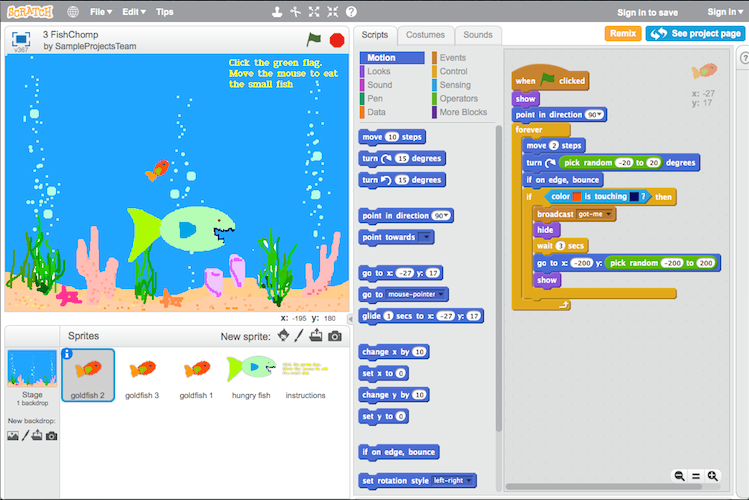
\includegraphics[scale=0.85]{./pics/scratch_ui.png}
\caption{Scratch's visual interface}
\label{fig:scratch_environment}
\end{center}
\end{figure}

There exist other similar programming environments to Scratch, namely Greenfoot and Alice which also have the same purpose of introducing programming to people without prior experience, which also happens to make all three systems share the same design goals \cite{AliceGreenfootScratch}. They tend to support various graphics and sounds which facilitate in the building of programs. One key difference lies in the target group each platform is addressing. Both Alice and Greenfoot target older students than Scratch, while they emphasize on Java and its concepts by introducing class-based and object-oriented programming. Given this fact, Scratch is often used as an introduction to both Alice and Greenfoot.
\subsection{Alice}
Alice is 3-dimensional interactive animation environment which allows novice programmers to create animated 3D movies in order to get a better understanding of object-oriented programming concepts. Similarly to Scratch, it provides a drag-and-drop functionality in order to prevent syntactical errors which are prevalent for beginners. Working with such a 3D graphics environment is also highly motivating with work with given its visual nature and immediate feedback which helps the novices to see the impact of a statement or a group of such.
Additionally,  The 3D modeled classes and objects
provide a concrete notion of the concept of objects
and support an “object-first” approach. Alice was designed originally as a tool to improve undergraduate student's ability to succeed in CS1 while currently it is being adopted by hundreds of secondary schools and colleges for pre-CS1, CS1 and non-majors courses.\cite{Alicecourse} Alice's visual interface could be seen in Figure \ref{fig:alice_environment}
\begin{figure}[H]
\begin{center}
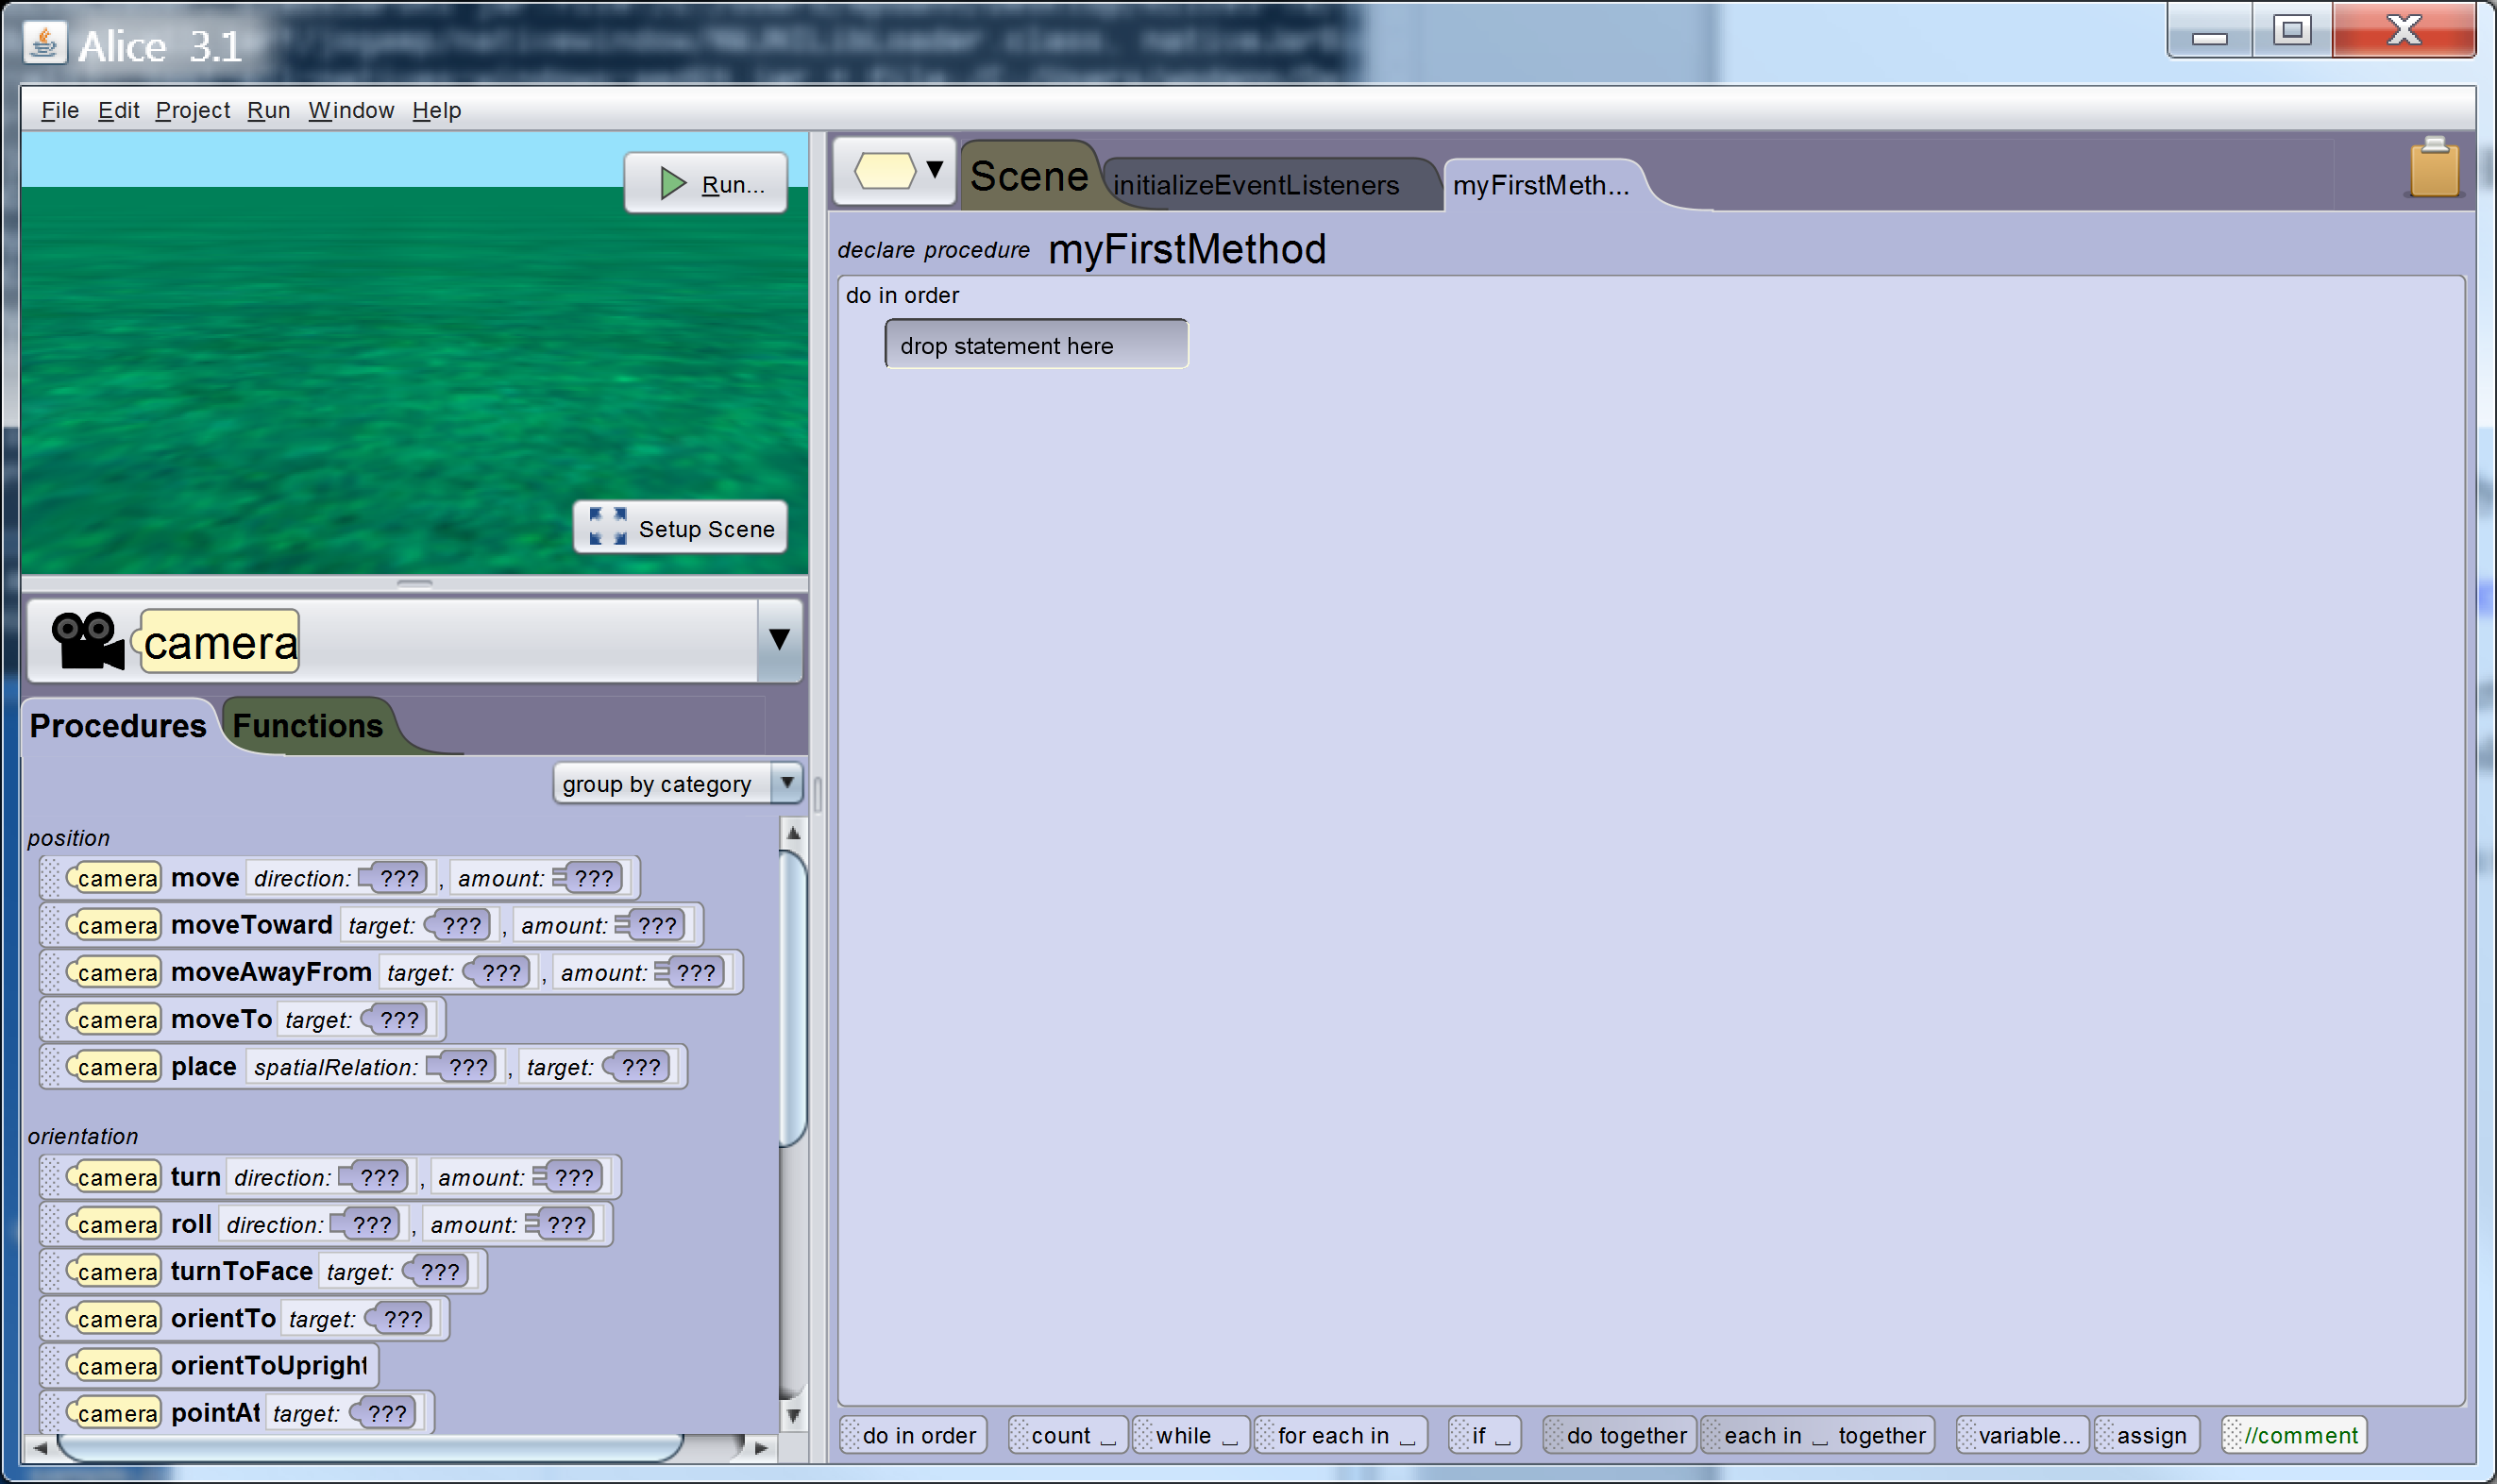
\includegraphics[scale=0.14]{./pics/Alice3D.png}
\caption{Alice's visual interface}
\label{fig:alice_environment}
\end{center}
\end{figure}
\subsection{Greenfoot}
As already mentioned, Greenfoot is a graphical environment which emphasises on the educational aspect of programming with Java. It gives the proper toolkit for developing engaging and interesting programs while using and learning more about object-orientation concepts. Transitioning from Scratch to Greenfoot is very smooth since the two platforms share similar features on of which is the direct mapping from Scratch's sprites and stage map to Greenfoot's actors and world. \cite{MaloneyResnick10}. The visual interface of Greenfoot can be seen on Figure \ref{fig:grenfoot_environment}.
\begin{figure}[H]
\begin{center}
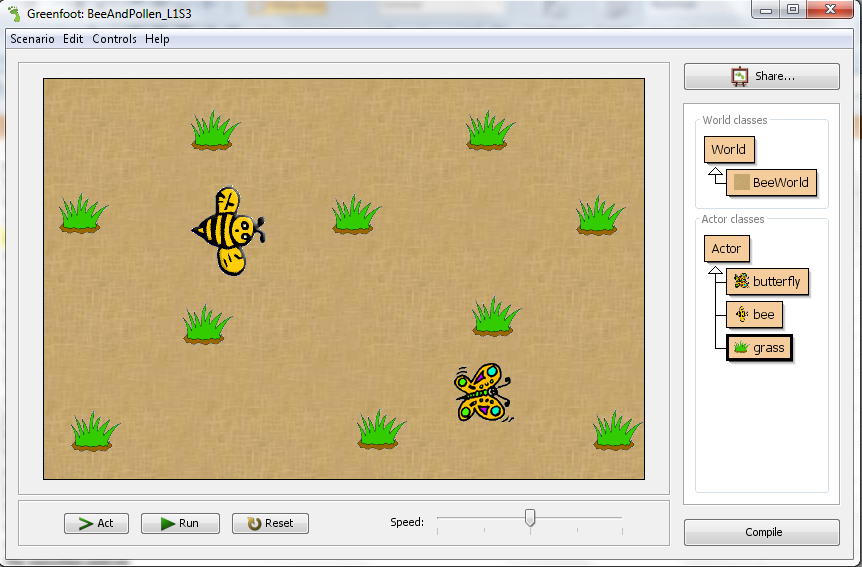
\includegraphics[scale=0.37]{./pics/greenfoot.png}
\caption{Greenfoot's visual interface}
\label{fig:grenfoot_environment}
\end{center}
\end{figure}


